\chapter{Architecture}

\begin{center}
\begin{figure}
  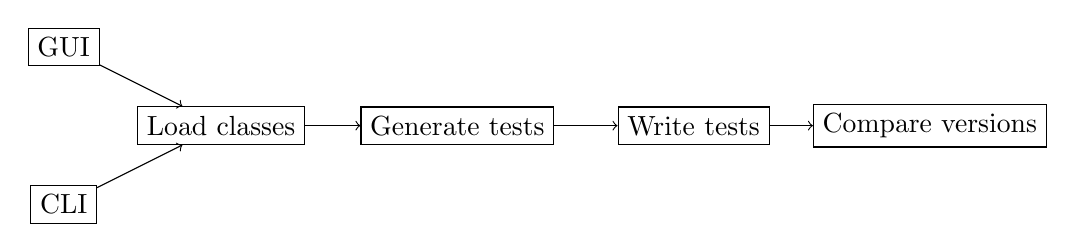
\begin{tikzpicture}
    \coordinate(origin);
    \node(core) at (origin) [draw] {Generate tests};
    \node(control) at ([left=3cm] core) [draw] {Load classes};
    \node(output) at ([right=3cm] core) [draw] {Write tests};
    \node(compare) at ([right=3cm] output) [draw] {Compare versions};
    \node(gui) at ([left=2cm,above=1cm] control) [draw] {GUI};
    \node(cli) at ([left=2cm,below=1cm] control) [draw] {CLI};

    \draw[->] (control) -> (core);
    \draw[->] (core) -> (output);
    \draw[->] (output) -> (compare);
    \draw[->] (gui) -> (control);
    \draw[->] (cli) -> (control);
  \end{tikzpicture}
\caption{A short summary of the control flow of SpLATS}
\label{fig:Architecture_HighLevel}
\end{figure}
\end{center}

  Ruby calls user-written libraries Gems, and there are many of these available. Once a program is finished, it can be bundled with all the Gems it used into one file which can be executed from any computer. The Gems used and the code that we wrote are discussed in this section.
  
  Figure \ref{fig:Architecture_HighLevel} shows the overall view of the system and figure \ref{fig:Architecture_LowLevel} shows SpLATS at a more in-depth level.

  \begin{center}
  \begin{figure}
  
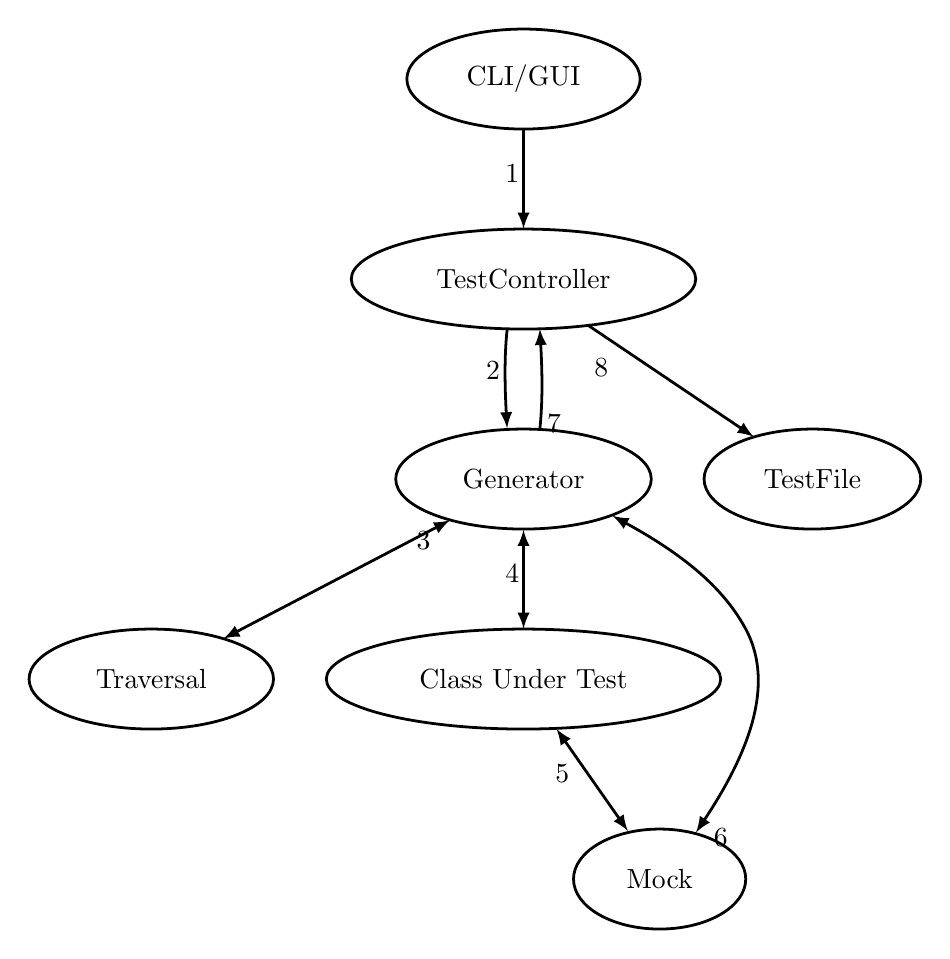
\begin{tikzpicture}[>=latex,line join=bevel,]
  \pgfsetlinewidth{1bp}
%%
\pgfsetcolor{black}
  % Edge: Generator -> TestController
  \draw [->] (183.91bp,180.28bp) .. controls (184.71bp,188.03bp) and (184.94bp,197.36bp)  .. (183.88bp,216.05bp);
  \definecolor{strokecol}{rgb}{0.0,0.0,0.0};
  \pgfsetstrokecolor{strokecol}
  \draw (189bp,182bp) node {7};
  % Edge: TestController -> TestFile
  \draw [->] (201.34bp,217.29bp) .. controls (216.4bp,207.16bp) and (236.12bp,193.88bp)  .. (260.86bp,177.23bp);
  \draw (206bp,202bp) node {8};
  % Edge: Class Under Test -> Mock
  \draw [<->] (189.86bp,72.055bp) .. controls (200.24bp,57.222bp) and (205.14bp,50.222bp)  .. (215.59bp,35.307bp);
  \draw (192bp,56bp) node {5};
  % Edge: CLI/GUI -> TestController
  \draw [->] (178bp,287.7bp) .. controls (178bp,279.98bp) and (178bp,270.71bp)  .. (178bp,252.1bp);
  \draw (174bp,272bp) node {1};
  % Edge: TestController -> Generator
  \draw [->] (172.12bp,216.05bp) .. controls (171.3bp,208.35bp) and (171.06bp,199.03bp)  .. (172.09bp,180.28bp);
  \draw (167bp,201bp) node {2};
  % Edge: Generator -> Class Under Test
  \draw [<->] (178bp,143.7bp) .. controls (178bp,128.69bp) and (178bp,123.49bp)  .. (178bp,108.1bp);
  \draw (174bp,128bp) node {4};
  % Edge: Generator -> Traversal
  \draw [<->] (151.53bp,147.17bp) .. controls (122.82bp,132.17bp) and (98.445bp,119.44bp)  .. (69.963bp,104.56bp);
  \draw (142bp,140bp) node {3};
  % Edge: Mock -> Generator
  \draw [<->] (240.08bp,34.735bp) .. controls (257.89bp,61.544bp) and (269.18bp,87.189bp)  .. (258bp,108bp) .. controls (249.58bp,123.68bp) and (234.26bp,135.5bp)  .. (210.02bp,148.79bp);
  \draw (249bp,33bp) node {6};
  % Node: CLI/GUI
\begin{scope}
  \definecolor{strokecol}{rgb}{0.0,0.0,0.0};
  \pgfsetstrokecolor{strokecol}
  \draw (178bp,306bp) ellipse (42bp and 18bp);
  \draw (178bp,306bp) node {CLI/GUI};
\end{scope}
  % Node: Generator
\begin{scope}
  \definecolor{strokecol}{rgb}{0.0,0.0,0.0};
  \pgfsetstrokecolor{strokecol}
  \draw (178bp,162bp) ellipse (46bp and 18bp);
  \draw (178bp,162bp) node {Generator};
\end{scope}
  % Node: Class Under Test
\begin{scope}
  \definecolor{strokecol}{rgb}{0.0,0.0,0.0};
  \pgfsetstrokecolor{strokecol}
  \draw (178bp,90bp) ellipse (71bp and 18bp);
  \draw (178bp,90bp) node {Class Under Test};
\end{scope}
  % Node: Traversal
\begin{scope}
  \definecolor{strokecol}{rgb}{0.0,0.0,0.0};
  \pgfsetstrokecolor{strokecol}
  \draw (44bp,90bp) ellipse (44bp and 18bp);
  \draw (44bp,90bp) node {Traversal};
\end{scope}
  % Node: TestController
\begin{scope}
  \definecolor{strokecol}{rgb}{0.0,0.0,0.0};
  \pgfsetstrokecolor{strokecol}
  \draw (178bp,234bp) ellipse (62bp and 18bp);
  \draw (178bp,234bp) node {TestController};
\end{scope}
  % Node: TestFile
\begin{scope}
  \definecolor{strokecol}{rgb}{0.0,0.0,0.0};
  \pgfsetstrokecolor{strokecol}
  \draw (282bp,162bp) ellipse (39bp and 18bp);
  \draw (282bp,162bp) node {TestFile};
\end{scope}
  % Node: Mock
\begin{scope}
  \definecolor{strokecol}{rgb}{0.0,0.0,0.0};
  \pgfsetstrokecolor{strokecol}
  \draw (227bp,18bp) ellipse (31bp and 18bp);
  \draw (227bp,18bp) node {Mock};
\end{scope}
%
\end{tikzpicture}


  \captionsetup{singlelinecheck=off}
  \caption[mock]{A more in-depth summary of the control flow of SpLATS
    \begin{enumerate}
      \item The user starts a UI of their choice, and passes in the file or files to be tested, a directory to put the finished tests, a traversal method and any parameters for that method. The interface then starts the TestController, which creates the output directory if one is needed, and loads the input files and their relevant classes.
      \item The TestController initialises a Generator for each class, with the traversal method and parameters.
      \item The Generator and Traversal methods determine how tests should be generated.
      \item Once the tests are produced, the Generator executes the test for the class.
      \item The Class Under Test calls methods on MockObjects that it is passed by the Generator.
      \item The MockObject asks the Generator for primitive values, or for a new MockObject to return to the CUT.
      \item The Generator yields the Test to the TestController.
      \item The tests are written to disk using the TestFile class.
    \end{enumerate}
  }
  \label{fig:Architecture_LowLevel}
  \end{figure}
  \end{center}
  
  \section{Gems used}
  \paragraph{Green Shoes} The GUI framework.
  \paragraph{Graph} Used to draw graphs.
  \paragraph{SimpleCov} Used in conjunction with Test::Unit to determine how much of the code the tests test. It produces an HTML file of the percentage of code covered, and displays it in a nice format.
  \paragraph{FlexMock} Used in the generated tests to test the execution path through the methods being tested.
  \paragraph{Yard} Used to automatically generate documentation.
  
  \section{User Interface}
  \subsection{Command Line Interface (CLI)}
  
  The CLI is a simple wrapper used to interact with SpLATS. 
  It uses the built-in Ruby OptionParser class, which allowed us to specify and analyse the options that the user enters. 
  The CLI's purpose is to read the entered arguments, create a traversal object, and pass the relevant file and output directory to the TestController.
  As only text commands are used as input, a user can easily automate the testing process with a script, so that many test can be executed at once.
  If the user enters an invalid command then the CLI will show an error messsage along with an explanation of the commands.
  The commands below are taken from the message displayed to the user when running without arguments.
  \begin{figure}
  \scriptsize
  \begin{verbatim}
Usage: splats [options]
  -h, --help                       Display help screen
  -G, --generate                   Generate a set of tests for the given file
  -C, --compare                    Generate a set of tests based on the first file, and then run those tests
                                    on the second file
  -f, --object-from-file FILE      Test classes from file. File & class must share names
  -g FILE,                         Second test classes from file. File & class must share names
      --comparee-object-from-file
  -o, --output-directory DIR       Output directory (defaults to "tests/") Fails if directory already exists
  -O, --output-directory-force DIR Output directory (defaults to "tests/") May overwrite if directory already
                                    exists
  -d, --depth [DEP]                Use depth limited traversal with search space provided depth DEP (default 3)
  -r, --random [SEED]              Use random traversal with provided SEED (default random)
  -m, --manual                     Use manual traversal
  \end{verbatim}
  \caption{CLI commands}
  \end{figure}
  \subsection{Graphical User Interface (GUI)}
  \subsubsection{Choice of framework}
  When researching which GUI to use, the vast majority of those for Ruby are either no longer supported, have a non-native look about them, or work only with Mac or Windows. Since the majority of the group are Unix users, the latter constraint meant that there were only a few to choose from. There is a page on wikipedia comparing the various frameworks on offer\footnote{\url{http://en.wikibooks.org/wiki/Ruby_Programming/GUI_Toolkit_Modules}}, and from this page (and other forums) Ruby Shoes unanimously stood out as it is extremely quick to load elements and has a shallow learning curve.
  Shoes\footnote{\url{http://shoesrb.com/}} is a stand-alone program which comes shipped with its own version of Ruby. After it was decided to use Gems for bundling, the GUI was ported to Green Shoes\footnote{\url{https://github.com/ashbb/green_shoes}}.
  
  \subsubsection{Design}
  The GUI was designed to be minimalist with as few buttons as possible. As no one in the group proclaimed to be a designer, the look of the GUI is minimalist as well. The images are used to illustrate the what the user sees on execution of the GUI.
  
  Figure \ref{fig:GUI_Page1} shows the first page. The button \verb+Load first version of the code+ is all that is displayed, giving only one option: to load the version of the code to run tests for. The preferred design would have been to pop up the file dialog box without clicking this button, but Green Shoes has many bugs which are difficult to overcome, and this was one of them. There is no other information on the first page, because it is assumed that the user wants to just begin testing and they already know what the program does. The \verb+file open+ dialog will not allow the user to cancel, nor allow the user to select a file which isn't '.rb'. Once a valid file is loaded, the \verb+next+ button and the text box appear. The text box is there to show the user what the inside of the file looks like, just so they are certain that they have loaded the correct version to test. There is a bug in Green Shoes, where the scroll bar doesn't appear on these text boxes, however they are scrollable with the mouse. The issues encountered with Green Shoes will be discussed in the "Problems" section. In future implementations of SpLATS, it would be possible to make this file box editable and writeable, but that is not high on the list of priorities.
Figure \ref{fig:GUI_Page2} is the same as the first page, only for the second version of the code.
  
  \begin{figure}
    \centering
    \subfloat[Load version 1]{\label{fig:GUI_Page1}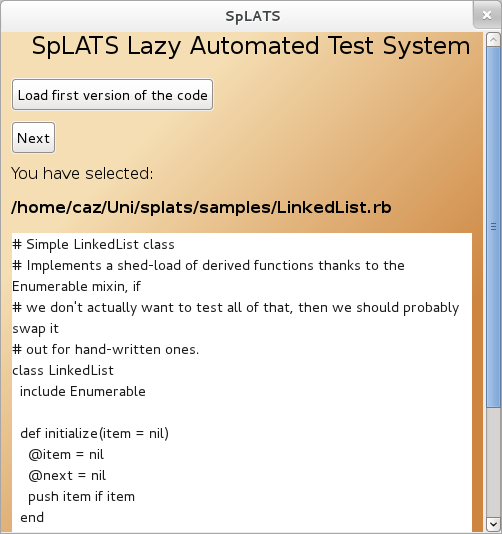
\includegraphics[width=0.4\textwidth]{page_1}}                
    \subfloat[Load version 2]{\label{fig:GUI_Page2}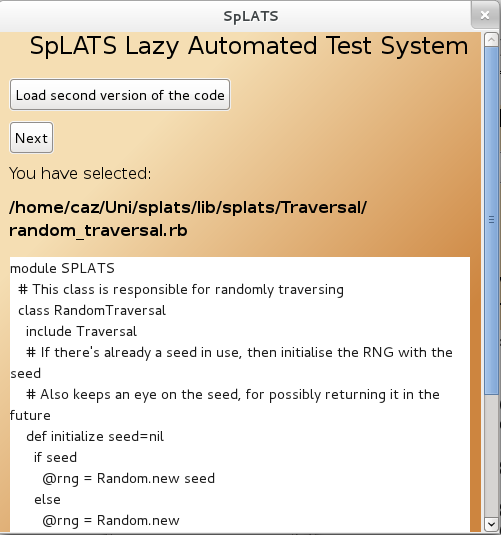
\includegraphics[width=0.4\textwidth]{page_2}}
    \caption{These pages are displayed when the user loads files to test}
    \label{fig:GUI_LoadVersions}
  \end{figure}
  
  Figure \ref{fig:GUI_Page3a} show the options the user then has to traverse the code. As discussed in the traversal methods, SpLATS currently only implements three traversal methods, but more can be added easily into the GUI. As the user changes their selection in the drop-down box, the options in the space below change to update inputs. Figures \ref{fig:GUI_Page3b} and \ref{fig:GUI_Page3c} illustrate this. The "next" button on third page doesn't do anything unless the extra parameters for "Random" and "Depth-Limited" are correct. Figure \ref{fig:GUI_Page3d} shows what the user sees when they've entered an invalid seed.
  
  \begin{figure}
    \centering
    \subfloat[Default traversal page]{\label{fig:GUI_Page3a}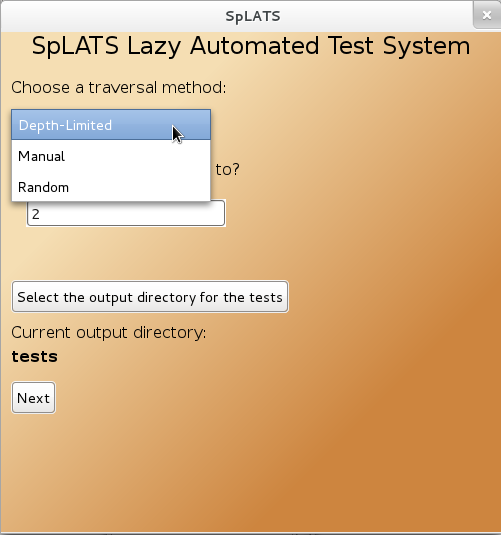
\includegraphics[width=0.4\textwidth]{page_3a}}
    \subfloat[Traversal options]{\label{fig:GUI_Page3b}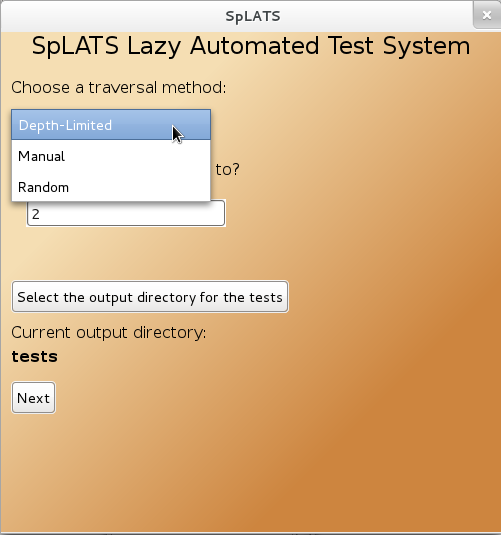
\includegraphics[width=0.4\textwidth]{page_3b}}
    \caption{The page the user sees when selecting a traversal method}
    \label{fig:GUI_SelectTraversal1}
  \end{figure}
  
  \begin{figure}
    \centering
    \subfloat[Random traversal]{\label{fig:GUI_Page3c}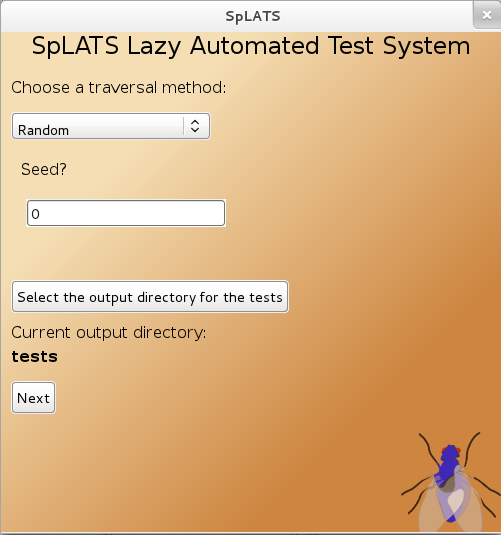
\includegraphics[width=0.4\textwidth]{page_3c}}
    \subfloat[Error in input]{\label{fig:GUI_Page3d}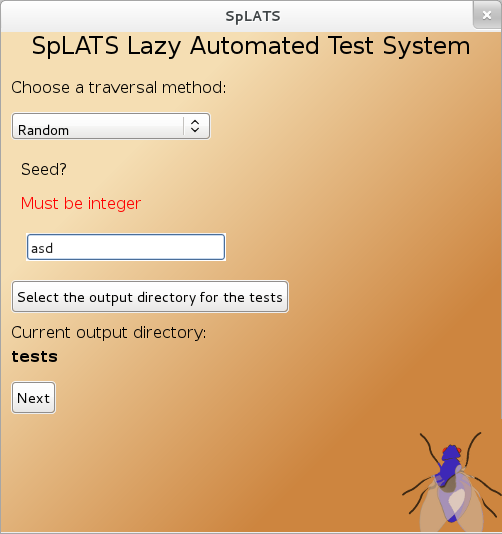
\includegraphics[width=0.4\textwidth]{page_3d}}
    \caption{Traversal page}
    \label{fig:GUI_SelectTraversal2}
  \end{figure}
  
  Once the user has input the correct information and they click "next", if they have selected "depth-limited" or "random" as the traversal methods, they will only see a page saying "generating tests", an alert pops up saying "testing complete" and SpLATS GUI will exit. It was decided not to draw graphs for these methods because the graphs will be extremely large.
  
  If the user has selected "Manual", then the GUI becomes more interesting. In order to have the GUI communicating with the code running SpLATS, threads were initially chosen. In theory, one thread would start the SpLATS process, and then when the user needed to give input, the thread would switch back to the GUI to ask for the user, the user would give input and so on until the end of the generation. The problem with threads is that they are determined by the thread scheduler, and it is difficult to time the threads and dictate exactly which thread should start when. This problem was overcome by using Ruby's in-built Fiber module. This is a much more lightweight implementation of Threads, but they don't need a scheduler, each Fiber has its own stack and the Fibers need to be specifically started and stopped. The three of these in combination were exactly what was needed to make the GUI run. Without the overhead of a scheduler, the GUI is extremely lightweight. The stack means that variables could be passed between Fibers, so the options available to the user are sent from the controller to the GUI, and the user's choice sent from the GUI to the controller. Figure \ref{fig:GUI_Page4a} shows the first choice the user will always have when in manual mode. They have to select which parameters to give to the initialise method (if there are any). When debugging the human traversal in the CLI, the context of the decision being made was difficult to deduce. The design decision was made to show the user the relevant line in the code, plus or minus five lines.
  
  \begin{figure}
    \centering
    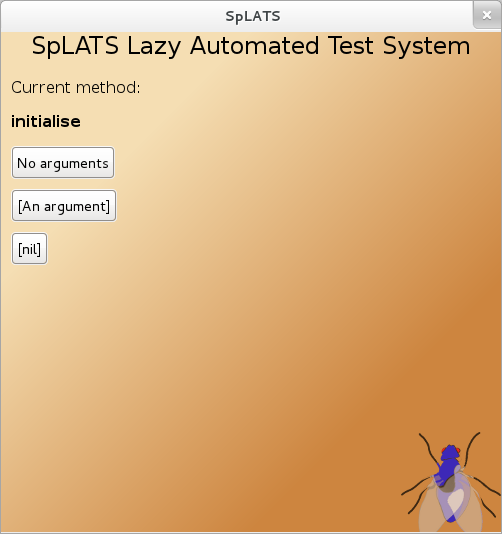
\includegraphics[width=0.5\textwidth]{page_4a}
    \caption{Manual traversal: "initialise" parameter choice}
    \label{fig:GUI_Page4a}
  \end{figure}
  
  \begin{figure}
    \centering
    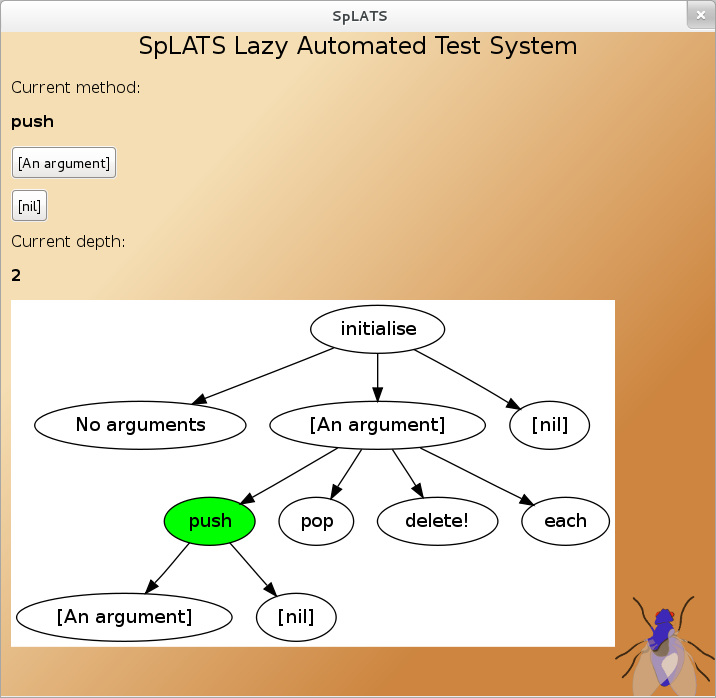
\includegraphics[width=0.8\textwidth]{page_4b}
    \caption{Manual traversal: "choose method" graph display of previous selections}
    \label{fig:GUI_Page4b}
  \end{figure}
  
  As the user steps down the traversal tree, they are presented a graph at each choice they have the option to make. A new window pops up, displaying a graph generated from information stored in SpLATS as the user makes their selections. The graph was designed to be a maximum of three levels deep, because otherwise displaying the user the information becomes too cumbersome. Figure \ref{fig:GUI_Page4b} shows what the user sees when they have already made decisions, and they are being asked to select the next method to generate tests for. This way the user can keep track of the methods they have selected and at what depth they are currently at.

  \section{Test Generator}
    The purpose of the test generator is to produce tests for a given Class
Under Test (CUT). The generator is also passed a traversal object which is used
to direct the generator's search.

    The production of tests in SpLATS can be visualised as a tree where each
node represents a choice that must be made. The choices in question are which
method to test; the values of the arguments to pass to that method; and any primitive
values that must be created (termed 'MockDecisions') during the execution of the CUT. A primitive value is defined as those classes which are built into Ruby (e.g. String, Integer, Boolean, etc.).
    The test can be considered as being split into individual TestLines each comprising one
method, one set of arguments, and multiple mock decisions.

%TODO: Insert tree diagram

    Each time a decision node is reached, the Generator offers a selection of options to the Traversal object. The Traversal method is responsible for tracking and directing the execution path in the manner it deems best.
    
    \paragraph{Method selection} Initially, the CUT must be constructed. Lightweight Ruby assumes the only way of doing so is through the class' \texttt{new} method. This is given to the Traversal class as the only option for updating its internal state. In subsequent iterations, Ruby's in-built reflection libraries are used to retrieve the possible callable public methods on the object.
    
    \paragraph{Argument selection} The chosen method's signature is examined and all possible sets of arguments are determined, taking into consideration required and optional parameters. The only arguments which can be chosen are nil or Mock.
    
    \paragraph{TestLine} TestLine is executed and the result is recorded. Any Mock objects which were passed into the method record any methods called upon them. They are thus able to trace the execution path from input to output. This solution aims to solve the problems associated with determining acceptable input types under Ruby's duck-typing. After each TestLine or Test is generated, the Traversal object is queried to see if another line should be generated.
    
    \paragraph{MockDecision} Under most circumstances, a methoc call made on a Mock object will return either a new Mock object or nil. Some method calls on a Mock object are defined as returning primitive types, as this is what Ruby expects in situations such as numerical operations or type casts. This return of a primitive type also helps to prevent an infinite chain of Mocks being created. Each time one of these primitive values is returned, other options available at that branch point are added to the Traversal search space.    
    
    \paragraph{Pruning} If the execution of a line raises an error, further descent of the tree will be halted, and the Traversal object is notified of the Exception. This is the only form of pruning SpLATS currently implements. Further improvements of SpLATS could prune by checking that isomorphic test cases, or similar cases are not being created. 

    \paragraph{Implemented Traversal Methods} Three traversal methods have so far been written: Depth-Limited, Manual and Random. The comparison between these methods can be found in the Evaluation section. The interface has been designed so that it is easy to write new traversal methods and primitive data generators.

  \subsection{Output}
    When tests are generated by the Generator, they are added line-by-line to a Test object which stores them in a class called TestLine. If SpLATS is only generating tests from a single input file, then the Test object is passed to TestFile. TestFile is a wrapper around Ruby's in-built IO::File and is used to write the tests to file. If SpLATS is performing regression testing, the files are not written to disk, but are generated and run in memory.
    
    Initially all the Tests were stored until the Generator had finished, but the Tests store all the Mock objects associated with them and this caused many out-of-memory errors. This was therefore changed so the Tests could be garbage-collected as soon as possible.
    
    The tests are output as Test::Units. When these tests are run, FlexMock is used to ensure that calls are made upon the inputs of functions and to track the source of the outputs.
